\chapter{Lumpy}

\label{lumpy}



Throughout the book, I have used diagrams to represent the state of

running programs.

\index{Lumpy}



In Section~\ref{variables}, we used a state diagram to show the names

and values of variables.  In Section~\ref{stackdiagram} I introduced a

stack diagram, which shows one frame for each function call.  Each

frame shows the parameters and local variables for the function or

method.  Stack diagrams for recursive functions appear in

Section~\ref{recursive.stack} and Section~\ref{more.recursion}.

\index{stack diagram} \index{diagram!stack}

\index{state diagram} \index{diagram!state}



Section~\ref{mutable} shows what a list looks like in a state diagram,

Section~\ref{invert} shows what a dictionary looks like, and

Section~\ref{dictuple} shows two ways to represent tuples.



Section~\ref{attributes} introduces object diagrams, which show the

state of an object's attributes, and their attributes, and so on.

Section~\ref{rectangles} has object diagrams for Rectangles and

their embedded Points.  Section~\ref{time.object} shows the state

of a Time object.

Section~\ref{class.attribute} has a diagram that includes a class

object and an instance, each with their own attributes.

\index{object diagram}

\index{diagram!object}



Finally, Section~\ref{class.diagram} introduces class diagrams,

which show the classes that make up a program and the relationships

between them.

\index{class diagram}

\index{diagram!class}



These diagrams are based on the Unified Modeling Language (UML), which

is a standardized graphical language used by software engineers

to communicate about program design, especially for object-oriented

programs.

\index{Unified Modeling Language}

\index{UML}



UML is a rich language with many kinds of diagrams that represent

many kinds of relationship between objects and classes.  What I presented

in this book is a small subset of the language, but it is the subset

most commonly used in practice.



The purpose of this appendix is to review the diagrams presented in

the previous chapters, and to introduce Lumpy.  Lumpy, which stands

for ``UML in Python,'' with some of the letters rearranged, is part of

Swampy, which you already installed if you worked on the case study in

Chapter~\ref{turtlechap} or Chapter~\ref{tkinter}, or if you did

Exercise~\ref{canvas},

\index{Lumpy}

\index{Swampy}



Lumpy uses Python's {\tt inspect} module to examine the state of a running

program and generate object diagrams (including stack diagrams) and

class diagrams.



\section{State diagram}



\begin{figure}

\centerline

{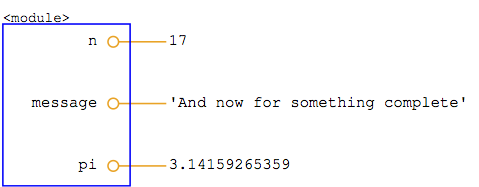
\includegraphics[scale=0.7]{figs/lumpydemo1.pdf}}

\caption{State diagram generated by Lumpy.}

\label{fig.lumpy1}

\end{figure}



Here's an example that uses Lumpy to generate a state diagram.

\index{state diagram} \index{diagram!state}



\begin{verbatim}

from swampy.Lumpy import Lumpy



lumpy = Lumpy()

lumpy.make_reference()



message = 'And now for something completely different'

n = 17

pi = 3.1415926535897932



lumpy.object_diagram()

\end{verbatim}



The first line imports the Lumpy class from {\tt swampy.Lumpy}.

If you don't have Swampy installed as a package, make sure

the Swampy files are in Python's search path and use this

{\tt import} statement instead:



\begin{verbatim}

from Lumpy import Lumpy

\end{verbatim}



The next lines create a {\tt Lumpy} object and make a ``reference''

point, which means that Lumpy records the objects that have been

defined so far.



Next we define new variables and invoke \verb"object_diagram",

which draws the objects that have been defined since the reference

point, in this case {\tt message}, {\tt n} and {\tt pi}.



Figure~\ref{fig.lumpy1} shows the result.  The graphical style is

different from what I showed earlier; for example, each

reference is represented by a circle next to the variable name and a

line to the value.  And long strings are truncated.  But the

information conveyed by the diagram is the same.



The variable names are in a frame labeled \verb"<module>", which

indicates that these are module-level variables, also known as

global.

\index{global variable}

\index{variable!global}

\index{module-level variable}

\index{variable!module-level}



You can download this example from

\url{http://thinkpython.com/code/lumpy_demo1.py}.  Try adding some

additional assignments and see what the diagram looks like.





\section{Stack diagram}



\begin{figure}

\centerline

{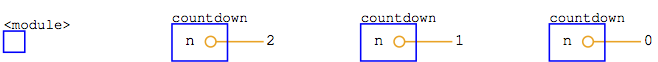
\includegraphics[scale=0.7]{figs/lumpydemo2.pdf}}

\caption{Stack diagram.}

\label{fig.lumpy2}

\end{figure}



Here's an example that uses Lumpy to generate a stack diagram.

You can download it from \url{http://thinkpython.com/code/lumpy_demo2.py}.

\index{stack diagram} \index{diagram!stack}



\begin{verbatim}

from swampy.Lumpy import Lumpy



def countdown(n):

    if n <= 0:

        print 'Blastoff!'

        lumpy.object_diagram()

    else:

        print n

        countdown(n-1)



lumpy = Lumpy()

lumpy.make_reference()

countdown(3)

\end{verbatim}



Figure~\ref{fig.lumpy2} shows the result.  Each frame is represented

with a box that has the function's name outside and variables inside.

Since this function is recursive, there is one frame for each

level of recursion.

\index{recursion}

\index{function frame}

\index{frame}



Remember that a stack diagram shows the state of the program at

a particular point in its execution.  To get the diagram you want,

sometimes you have to think about where to invoke \verb"object_diagram".



In this case I invoke \verb"object_diagram" after executing the base

case of the recursion; that way the stack diagram shows each level of

the recursion.  You can call \verb"object_diagram" more than once to

get a series of snapshots of the program's execution.

\index{base case}





\section{Object diagrams}



\begin{figure}

\centerline

{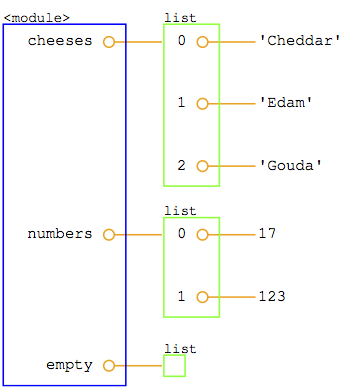
\includegraphics[scale=0.7]{figs/lumpydemo3.pdf}}

\caption{Object diagram.}

\label{fig.lumpy3}

\end{figure}



This example generates an object diagram showing the lists from

Section~\ref{sequence}.  You can download it from

\url{http://thinkpython.com/code/lumpy_demo3.py}.

\index{object diagram} \index{diagram!object}



\begin{verbatim}

from swampy.Lumpy import Lumpy



lumpy = Lumpy()

lumpy.make_reference()



cheeses = ['Cheddar', 'Edam', 'Gouda']

numbers = [17, 123]

empty = []



lumpy.object_diagram()

\end{verbatim}



Figure~\ref{fig.lumpy3} shows the result.  Lists are represented by

a box that shows the indices mapping to the elements.  This representation

is slightly misleading, since indices are not actually

part of the list, but I think they make the diagram easier to

read.  The empty list is represented by an empty box. 

\index{list index}



\begin{figure}

\centerline

{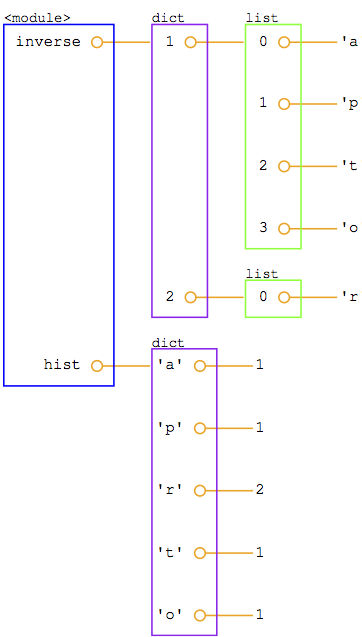
\includegraphics[scale=0.7]{figs/lumpydemo4.pdf}}

\caption{Object diagram.}

\label{fig.lumpy4}

\end{figure}



And here's an example 

showing the dictionaries from Section~\ref{invert}.  You can download

it from \url{http://thinkpython.com/code/lumpy_demo4.py}.

\index{dictionary}



\begin{verbatim}

from swampy.Lumpy import Lumpy



lumpy = Lumpy()

lumpy.make_reference()



hist = histogram('parrot')

inverse = invert_dict(hist)



lumpy.object_diagram()

\end{verbatim}



Figure~\ref{fig.lumpy4} shows the result.  {\tt hist} is a dictionary

that maps from characters (single-letter strings) to integers;

{\tt inverse} maps from integers to lists of strings.



\begin{figure}

\centerline

{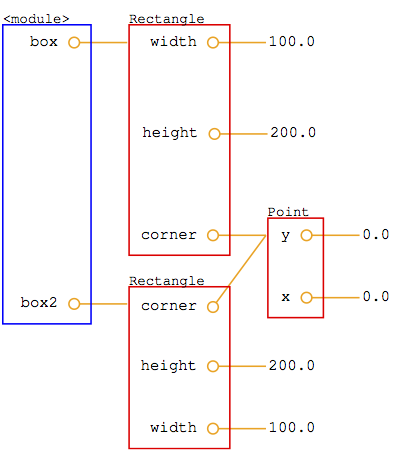
\includegraphics[scale=0.7]{figs/lumpydemo5.pdf}}

\caption{Object diagram.}

\label{fig.lumpy5}

\end{figure}



This example generates an object diagram for Point and Rectangle

objects, as in Section~\ref{copying}.  You can download it from

\url{http://thinkpython.com/code/lumpy_demo5.py}.

\index{Point class}

\index{class!Point}

\index{Rectangle class}

\index{class!Rectangle}



\begin{verbatim}

import copy

from swampy.Lumpy import Lumpy



lumpy = Lumpy()

lumpy.make_reference()



box = Rectangle()

box.width = 100.0

box.height = 200.0

box.corner = Point()

box.corner.x = 0.0

box.corner.y = 0.0



box2 = copy.copy(box)



lumpy.object_diagram()

\end{verbatim}



Figure~\ref{fig.lumpy5} shows the result.  {\tt copy.copy} make a

shallow copy, so {\tt box} and {\tt box2} have their own {\tt width}

and {\tt height}, but they share the same embedded Point object.  This

kind of sharing is usually fine with immutable objects, but with

mutable types, it is highly error-prone.

\index{copy}

\index{shallow copy}



\section{Function and class objects}



\begin{figure}

\centerline

{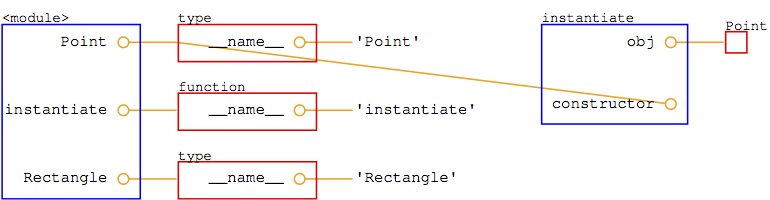
\includegraphics[scale=0.7]{figs/lumpydemo6.pdf}}

\caption{Object diagram.}

\label{fig.lumpy6}

\end{figure}



When I use Lumpy to make object diagrams, I usually define the functions

and classes before I make the reference point.  That way, function

and class objects don't appear in the diagram.

\index{function object}

\index{object!function}

\index{class object}

\index{object!class}



But if you are passing functions and classes as parameters, you might

want them to appear.  This example shows what that looks like;

you can download it from

\url{http://thinkpython.com/code/lumpy_demo6.py}.



\begin{verbatim}

import copy

from swampy.Lumpy import Lumpy



lumpy = Lumpy()

lumpy.make_reference()



class Point(object):

    """Represents a point in 2-D space."""



class Rectangle(object):

    """Represents a rectangle."""



def instantiate(constructor):

    """Instantiates a new object."""

    obj = constructor()

    lumpy.object_diagram()

    return obj



point = instantiate(Point)

\end{verbatim}



Figure~\ref{fig.lumpy6} shows the result.  Since we invoke

\verb"object_diagram" inside a function, we get a stack diagram

with a frame for the module-level variables and for the invocation

of {\tt instantiate}.



At the module level, {\tt Point} and {\tt Rectangle} refer to

class objects (which have type {\tt type}); {\tt instantiate}

refers to a function object.

\index{instantiate}

\index{constructor}



This diagram might clarify two points of common confusion: (1) the

difference between the class object, {\tt Point}, and the instance of

Point, {\tt obj}, and (2) the difference between the function object

created when {\tt instantiate} is defined, and the frame created with

it is called.





\section{Class Diagrams}



\begin{figure}

\centerline

{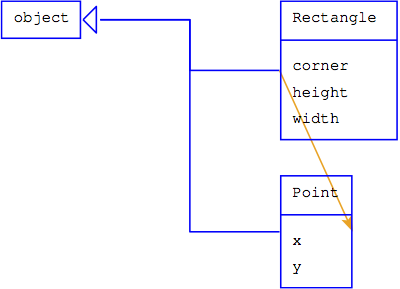
\includegraphics[scale=0.7]{figs/lumpydemo7.pdf}}

\caption{Class diagram.}

\label{fig.lumpy7}

\end{figure}



\begin{figure}

\centerline

{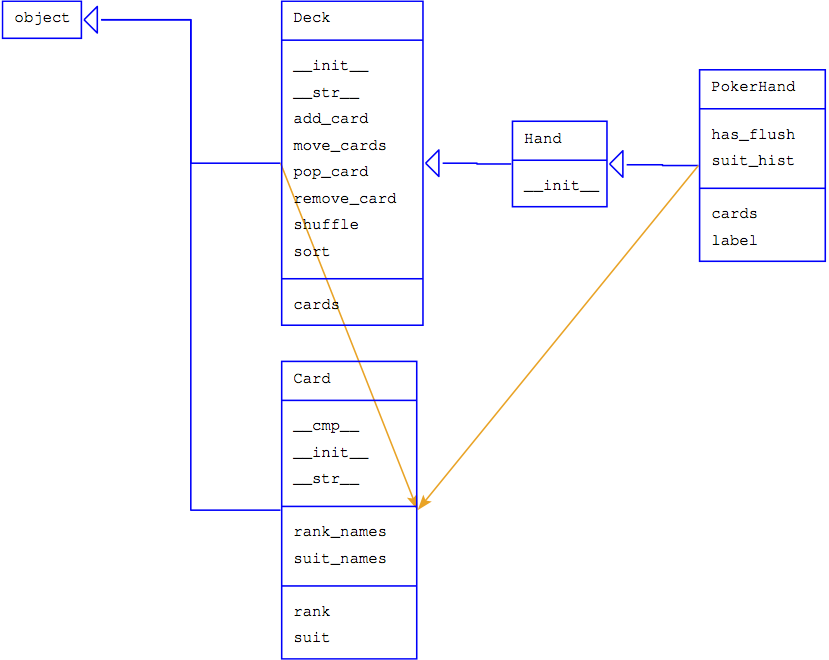
\includegraphics[scale=0.7]{figs/lumpydemo8.pdf}}

\caption{Class diagram.}

\label{fig.lumpy8}

\end{figure}



Although I distinguish between state diagrams, stack diagrams and

object diagrams, they are mostly the same thing: they show the

state of a running program at a point in time.

\index{class diagram}

\index{diagram!class}



Class diagrams are different.  They show the classes that make up a

program and the relationships between them.  They are timeless in the

sense that they describe the program as a whole, not any particular

point in time.  For example, if an instance of Class A generally

contains a reference to an instance of Class B, we say there is a

``HAS-A relationship'' between those classes.

\index{HAS-A relationship}

\index{class diagram}

\index{diagram!class}

\index{UML}



Here's an example that shows a HAS-A relationship.  You can download

it from \url{http://thinkpython.com/code/lumpy_demo7.py}.



\begin{verbatim}

from swampy.Lumpy import Lumpy



lumpy = Lumpy()

lumpy.make_reference()



box = Rectangle()

box.width = 100.0

box.height = 200.0

box.corner = Point()

box.corner.x = 0.0

box.corner.y = 0.0



lumpy.class_diagram()

\end{verbatim}



Figure~\ref{fig.lumpy7} shows the result.  

Each class is represented with a box that contains the name of the

class, any methods the class provides, any class variables, and

any instance variables.  In this example, {\tt Rectangle} and {\tt Point}

have instance variables, but no methods or class variables.



The arrow from {\tt Rectangle} to {\tt Point} shows that Rectangles

contain an embedded Point.  In addition, {\tt Rectangle} and {\tt

  Point} both inherit from {\tt object}, which is represented in

the diagram with a triangle-headed arrow.

\index{IS-A relationship}



Here's a more complex example using my solution to Exercise~\ref{poker}.

You can download

the code from \url{http://thinkpython.com/code/lumpy_demo8.py};

you will also need \url{http://thinkpython.com/code/PokerHand.py}.



\begin{verbatim}

from swampy.Lumpy import Lumpy



from PokerHand import *



lumpy = Lumpy()

lumpy.make_reference()



deck = Deck()

hand = PokerHand()

deck.move_cards(hand, 7)



lumpy.class_diagram()

\end{verbatim}



Figure~\ref{fig.lumpy8} shows the result.  

{\tt PokerHand} inherits from {\tt Hand}, which inherits from {\tt Deck}.

Both {\tt Deck} and {\tt PokerHand} have Cards.

\index{Card class}

\index{Deck class}

\index{Hand class}



This diagram does not show that {\tt Hand} also has cards, because

in the program there are no instances of Hand.  This example

demonstrates a limitation of Lumpy; it only knows about the

attributes and HAS-A relationships of objects that are instantiated.



\printindex



\clearemptydoublepage

%\blankpage

%\blankpage

%\blankpage





\end{document}
